\documentclass[10pt,twoside]{book}
\usepackage{../../thesis}
\graphicspath{ {../../images/} }

\makeindex
\begin{document}
\chapter{Symbolic Dynamics}
\label{chap:symbolic}
Recall that in Chapter~\ref{chap:devaney}, we postponed the proof that the doubling map is chaotic.
In the present chapter, we complete the proof using a technique called the \textit{symbolic dynamics}.
Then, we present a definition of chaos by Block and Coppel, which is motivated by symbolic dynamics.
%%%

\section{Shift Systems}
In the previous chapters, our examples consisted of simple yet tangible mappings such as the logistic map and tent map.
Now, we turn our attention to the dynamics of \textit{symbols}, an abstract system that might appear to be of little use at first sight.
Nevertheless, symbolic dynamical systems have rich structures and are not only interesting in its own right, but also useful tools for studying other systems, as we will demonstrate in the next section.
The particular system that we discuss is called the \textit{one-sided shift}.
The goal of this section is to prove that the full one-sided shift is chaotic in Devaney's sense.
\begin{definition}
  (One-sided shift)
  Let $S$ be a set of finite number of symbols, and let $\Sigma$ be a set of infinite sequences of the form
  \begin{equation*}
    s = \set{ s_0 s_1 s_2 \cdots s_n \cdots },
  \end{equation*}
  where $s_i \in S$.
  In other words, $\Sigma \ceq S^\N$.
  Although the symbols can be anything (Roman alphabets, colors, Chinese characters, etc.), we take a finite number of integers as our symbols.
  Thus, $S \ceq \set{1, \ldots, n}$.
  We put the absolute value metric on $S$.
  Then, define the metric on $\Sigma$ as follows:
  \begin{equation*}
    d(a,b) \ceq \sum\limits_{i = 0}^{\infty} \frac{\abs{a_i - b_i}}{2^i}.
  \end{equation*}
  Thus, two infinite sequences are close to each other if they agree on a long frontal block.
  The metric induces the topology on $\Sigma$.
  Let $\sigma: \Sigma \to \Sigma$ defined as:
  \begin{equation*}
    \sigma: \set{ s_0 s_1 s_2 \cdots s_n \cdots } 
    \mapsto 
    \set{ s_1 s_2 \cdots s_n \cdots }.
  \end{equation*}
  Thus, $\sigma$ corresponds to dropping the first symbol of the sequence, and shifting all other symbols to the front.
  When the space is $\Sigma$, which consists of all possible infinite sequences of symbols, we call the dynamical system ($\Sigma$, $\sigma$) the \textit{full one-sided shift}.
  If $X$ is a (appropriately chosen) subset of $\Sigma$, then $(X, \sigma)$ is called a \textit{subshift}.
  \index{one-sided shift}
\end{definition}
For the definition of a subshift to make sense, $X$ must be an invarient set of $\sigma$, but it is not the only requirement.
$X$ also needs to be closed in $\Sigma$.
Subshifts provide rich examples of dynamical systems, but we do not discuss them here.
For discussions on subshifts refer to \citet{kitchens} and \citet{lind}.
%%%

Before we proceed further, we prove that $d$ is a metric and $\sigma$ is a continuous map to ensure that it defines a topological dynamical system.
We also study the topology on $\Sigma$.
\begin{proposition}
  $d$ is a metric.
  \label{prop:symb-metric}
  \begin{proof}
    Clearly, $d(a,b) \geq 0$ for each $a,b \in \Sigma$.
    If $a = b$ then $d(a,b) = 0$.
    On the other hand, if $d(a,b) = 0$, then $a_i = b_i$ for each $i$, so we have $a = b$.
    Thus, we are left to prove the triangle inequality.
    Suppose $a,b,c \in \Sigma$.
    We have
    \begin{align*}
      d(a,b) + d(b,c)
      &\equiv \sum\limits_{i = 0}^{\infty} \frac{\abs{a_i - b_i}}{2^i}  +  \sum\limits_{i = 0}^{\infty} \frac{\abs{b_i - c_i}}{2^i}  \\
      %
      &= \sum\limits_{i = 0}^{\infty} \frac{\abs{a_i - b_i} + \abs{b_i - c_i}}{2^i}  \\
      %
      &\geq \sum\limits_{i = 0}^{\infty} \frac{\abs{a_i - c_i}}{2^i}  \\
      &= d(a,c).
    \end{align*}
  \end{proof}
\end{proposition}
%%%
It suffices for our purpose to use $S \ceq \set{0,1}$.
All properties of $(\Sigma, \sigma)$ that we prove in this section also hold when $S$ is any finite set of symbols, and letting $S$ consist of only two symbols greatly simplify proofs.
Also, we will not require more than two symbols for studying systems in this exposition.
Now, we prove two facts about our metric, which we use frequently.
\begin{proposition}
  Let $s, t \in \Sigma$.
  If $s_i = t_i$ for $0 \leq i \leq k$, then $d(s,t) \leq 2^{-k}$.
  \label{prop:symbol-bound1}
  \begin{proof}
    $d(s,t)$ achieves its maximum when $s_i \neq t_i$ for all $i \geq k+1$.
    \begin{equation*}
      d(s,t) 
      \leq \sum\limits_{i = k+1}^{\infty} \frac{1}{2^i}
      = \sum\limits_{i = 0}^{\infty} \frac{1}{2^i} - \sum\limits_{i = 0}^{k} \frac{1}{2^i}
      = 2 - (2 - \frac{1}{2^{k}})
      = 2^{-k}.
    \end{equation*}
  \end{proof}
\end{proposition}
Conversely, we can infer from the distance between the two the length of a block on which two sequences agree.
\begin{proposition}
  Let $s, t \in \Sigma$.
  If $d(s,t) < 2^{-k}$, then $s_i = t_i$ for $0 \leq i \leq k$.
  \label{prop:symbol-bound2}
  \begin{proof}
    If $s_i \neq t_i$ for any $0 \leq i \leq k$, then we would have
    \begin{equation*}
      d(s,t) \geq \frac{1}{2^i} \geq 2^{-k}.
    \end{equation*}
    Hence, it must hold that $s_i = t_i$ for each $0 \leq i \leq k$.
  \end{proof}
\end{proposition}
%%%
Next, we note the following properties of $S$, the set of finite symbols equipped with the absolute value metric.
\begin{proposition}
  $S$ equipped with the absolute value metric is 
  \begin{enumerate}[(i)]
    \item compact
    \item totally disconnected
  \end{enumerate}
  \begin{proof}
    \begin{enumerate}
      \item
        $S$ is finite.
        %%%
      \item 
        $S$ is a discrete space.
        Hence, it is totally disconnected.
        %%%
    \end{enumerate}
  \end{proof}
\end{proposition}
%%%
The topology of the underlying space are inherited to the space of infinite sequences of symbols, $\Sigma$, which is an infinite product of $S$.
\begin{proposition}
  $\Sigma$ equipped with the metric $d$ is 
  \begin{enumerate}[(i)]
    \item compact
    \item totally disconnected
    \item perfect.
  \end{enumerate}
  \begin{proof}
    \begin{enumerate}
      \item 
        It follows from Tychonov's theorem.
        %%%
      \item
        A product of totally disconnected space is also totally disconnected.
        See \citet{dugundji}.
        %%%
      \item
        Let $s$ an arbitrary member of $\Sigma$.
        We show that, for each $\epsilon > 0$, $\oball{\epsilon}{s}$ contains a point $t \neq s$.
        We may suppose that $2^{-k} < \epsilon$ for some $k \in \N$.
        Also suppose that
        \begin{align*}
          s = s_0 s_1 s_2 \cdots.
        \end{align*}
        Define $t$ by
        \begin{equation*}
          t_i = \begin{cases}
            &s_i \mbox{ if } 0 \leq i \leq k  \\
            &1 - s_i \mbox{ otherwise.}
          \end{cases}
        \end{equation*}
        Thus, $t$ agrees with $s$ on the first $k+1$ symbols, and differs after the $k+1$-th symbol.
        $t$ is clearly in $\Sigma$.
        Then, by Proposition~\ref{prop:symbol-bound1}, $d(s,t) \leq 2^{-k} < \epsilon$, so that $t \in \oball{\epsilon}{s}$.
        Hence, $\Sigma$ is perfect.
        %%%
    \end{enumerate}
  \end{proof}
\end{proposition}
%%%
Thus, $\Sigma$ is a \textit{Cantor set}.
Knowing the structure of $\Sigma$ will prove useful when we construct a conjugacy between the doubling map and the full one-sided shift.
Also, note that any dynamical system that is conjugate to the full one-sided shift possesses these properties of $\Sigma$ \citep{dugundji}.
%%%
Now we show that $\sigma$ is continuous and surjective.
\begin{proposition}
  ($\sigma$ is a homeomorphism)
  \begin{enumerate}[(i)]
    \item $\sigma$ is continuous.
    \item  $\sigma$ is surjective and two-to-one..
  \end{enumerate}
  \begin{proof}
    \begin{enumerate}[(i)]
      \item 
        Fix $\epsilon > 0$.
        We may assume that $2^{-k} < \epsilon$ for some positive integer $k$.
        For any $a \in \Sigma$, if $b \in \Sigma$ satisfies
        \begin{equation*}
          d(a,b) = \sum\limits_{i=0}^{\infty} \frac{\abs{a_i - b_i}}{2^i} < 2^{-(k+1)},
        \end{equation*}
        then 
        \begin{align*}
          d(\sigma(a), \sigma(b)) 
          &= \sum\limits_{i=1}^{\infty} \frac{\abs{a_i - b_i}}{2^i} 
          = \sum\limits_{i=0}^{\infty} \frac{\abs{a_i - b_i}}{2^i} - \abs{a_0 - b_0}  \\
          &< 2^{-(k+1)} - \abs{a_0 - b_0}
          < 2^{-k}
          < \epsilon.
        \end{align*}
        This shows that $\sigma$ is continuous.
        %%%
      \item  
        Each $s \in \Sigma$ takes the form
        \begin{equation*}
          s = s_0s_1s_2 \cdots.
        \end{equation*}
        $\sigma$ maps
        \begin{equation*}
          0 s_0s_1s_2 \cdots \mbox{ and } 1 s_0s_1s_2 \cdots
        \end{equation*}
        to $s$.
        Hence, $\sigma$ is surjective and two-to-one.
        %%%
    \end{enumerate}
  \end{proof}
  \label{prop:sigma-cont}
\end{proposition}
%%%
Finally, we show that $(X,\sigma)$ is chaotic.
\begin{theorem}
  %\citep{sternberg}
  The full one-sided shift is chaotic in Devaney's sense.
  \begin{proof}
    First, we prove that the dense periodic points of $\sigma$ is dense in $\Sigma$.
    Let $s$ be a member of $\Sigma$.
    Fix $\epsilon > 0$, and assume that $2^{-k} < \epsilon$ for some $k$.
    Then, construct $t \in \Sigma$ by letting $t_i = s_i$ for $0 \leq i \leq k$, and repeat $t_0 \cdots t_k$ afterwards, i.e.
    \begin{equation*}
      t = s_0 \cdots s_k s_0 \cdots s_k s_0 \cdots.
    \end{equation*}
    By Proposition~\ref{prop:symbol-bound1}, $d(s,t) \leq 2^{-k} < \epsilon$.
    Clearly, $t$ is periodic.
    Hence, each neighborhood of $s$ contains a periodic point.
    Since the choice of $s$ was arbitrary, we conclude that $P(\sigma)$ is dense in $\Sigma$.

    Next, we show that $\sigma$ is transitive.
    Fix $s,t \in \Sigma$.
    Also fix $\epsilon > 0$ and assume that $2^{-k} < \epsilon$ for some $k$.
    Consider a sequence
    \begin{equation*}
      s' = s_0 \cdots s_k t_0 t_1 t_2 \cdots.
    \end{equation*}
    Since $s'$ agrees $s$ for the first $k+1$ symbols, $s' \in \oball{\epsilon}{s}$.
    Note that we have
    \begin{equation*}
      \itr{\sigma}{k+1}(s') = t.
    \end{equation*}
    Hence, $\sigma$ is transitive.
  \end{proof}
\end{theorem}
%%%
It follows from Theorem~\ref{thm:silverman} that $(X, \sigma)$ is also sensitive to initial conditions.
However, we present a direct proof below, as symbolic dynamics provides a new perspective to our understanding of sensitive dependence on initial conditions.
\begin{proposition}
  The full one-sided shift is sensitive.
  \begin{proof}
    Fix $0 < \delta < 1$, the separation constant.
    Let $s$ be an arbitrary member of $\Sigma$, and for any $\epsilon > 0$, let $\oball{\epsilon}{s}$ be a neighborhood.
    Let $t \neq s$ be any point in $\oball{\epsilon}{s}$.
    We may suppose that $s_i \neq t_i$ for some $n \geq 0$.
    Then,
    \begin{equation*}
      \metric{\itr{\sigma}{n}(s), \itr{\sigma}{n}(t)} \geq 1 > \delta.
    \end{equation*}
  \end{proof}
\end{proposition}
%%%
The meaning of sensitive dependence on initial conditions is explicitly displayed in the proof.
A slight change in the initial conditions is represented as swapping symbols at positions deep down in the sequence.
We call the original sequence $x$ and the modified sequence $x'$.
Suppose $x$ and $x'$ differ \textit{only} at the $p$-th position.
We can think of $d(\itr{\sigma}{i}(x), \itr{\sigma}{i}(x'))$ as an error of some sort at the $i$-th time step.
As the system evolves, the $p$-th position comes closer and closer to the 0th position, and the error is doubled at each time step ($d(\sigma(x), \sigma(x')) = 2 \cdot d(x, x')$).
The error achieves its maximum after $p$ iterations.
After the $p+1$-th iteration, however, the error remains zero.
The situation is analogous to the behavior of a pair described in both Devaney's and Li-Yorke's definitions.
In Devaney's definition, for example, two nearby points separate by $\delta$, the separation constant, but they eventually come close to each other because of transitivity.
On the other hand, consider a situation where $x'$ agrees with $x$ up to the $k$-th position, but $x'_i$ for $i > k$ are randomly chosen.
Thus, $x'$ represents $x$ with some random noise.
As in the previous example, the error increases as the system evolves.
After the $k$-th iteration, $d(\itr{\sigma}{i}(x), \itr{\sigma}{i}(x'))$ is nothing but random, and does not tell us anything about $x$ and $x'$!
This observation motivates us to the metric $d'$ defined as
\begin{equation*}
  d'(s,t) = 2^{-k},
\end{equation*}
where $k$ is the first position at which $s$ and $t$ differ.
In fact, the metric that we use and this metric $d'$ can be shown to be equivalent metrics.
%%%

\section{Doubling Map is Chaotic}
The goal of this section is to prove that $(\Sigma, \sigma)$ is semi-conjugate to $(S^1, D)$, which implies that the doubling map is chaotic in Devaney's sense (Theorem~\ref{thm:conj-sdic}).
\begin{center}
  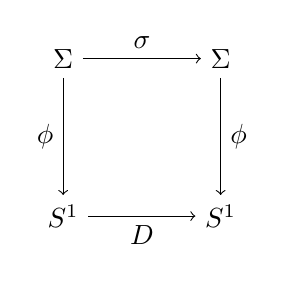
\begin{tikzpicture}[node distance=2cm, auto]
    \node (y1) {$\Sigma$};
    \node (y2) [right of=y1] {$\Sigma$};
    \node (x1) [below of=y1] {$S^1$};
    \node (x2) [below of=y2] {$S^1$};
    \draw[->] (x1) to node[swap] {$D$} (x2);
    \draw[->] (y1) to node[swap] {$\phi$} (x1);
    \draw[->] (y1) to node {$\sigma$} (y2);
    \draw[->] (y2) to node {$\phi$} (x2);
  \end{tikzpicture}
\end{center}
%%%
\begin{figure}[ht]
  \centering
  \begin{tikzpicture}[scale=3.2]
    \draw[->] (-0.2,0) -- (1.2,0) node[right] {$x$};
    \draw[->] (0,-0.2) -- (0,1.2) node[above] {$D(x)$};
    \foreach \x/\xtext in {0.5/\frac{1}{2}, 1/1}
    \draw[shift={(\x,0)}] (0pt,1pt) -- (0pt,-1pt) node[below] {$\xtext$};
    \foreach \y/\ytext in {0.5/\frac{1}{2}, 1/1}
    \draw[shift={(0,\y)}] (1pt,0pt) -- (-1pt,0pt) node[left] {$\ytext$};
    %%% graphs
    \draw[domain=0:0.492] plot (\x,{2*\x}) node[below right] {};
    \draw[domain=0.5:0.983] plot (\x,{2*\x - 1}) node[below right] {};
    \draw[] (0.99,0.99) circle (0.6pt);
    \draw[] (0.51,1) circle (0.6pt);
  \end{tikzpicture}
  \label{fig:doubling}
  \caption{The doubling map, $D(x)$.}
\end{figure}
%%%
The key to construct a semi-conjugacy between $(S^1,D)$ and $(\Sigma, \sigma)$ is to think of an infinite sequence in $\Sigma$ as the binary expansion of some real number.
As usual, we represent $S^1$ by an interval $[0,1)$, and for each $x \in S^1$, we consider its binary expansion, which is %]
\begin{equation*}
  x = \sum\limits_{i = 1}^{\infty} \frac{s_i}{2^i}.
\end{equation*}
Then, notice that
\begin{equation*}
  D(x) = 2 \cdot \sum\limits_{i = 1}^{\infty} \frac{s_i}{2^i}
  = \sum\limits_{i = 1}^{\infty} \frac{s_i}{2^{i-1}}
  = s_1 + \sum\limits_{i = 2}^{\infty} \frac{s_i}{2^{i-1}}
  = \sum\limits_{i = 2}^{\infty} \frac{s_i}{2^{i-1}}
  \quad(\mod{1}).
\end{equation*}
Therefore, if we represent each point in $S^1$ by its binary expansion, we can describe $D$ as follows
\begin{equation*}
  D: 0.s_1 s_2 s_3 \cdots \mapsto 0.s_2 s_3 \cdots,
\end{equation*}
which remind us of the shift map.
Motivated by this observation, we define a mapping $\phi: \Sigma \to S^1$, which assigns
\begin{equation*}
  \sum\limits_{i = 1}^{\infty} \frac{s_i}{2^i} \in S^1.
\end{equation*}
to
\begin{equation*}
  s_1 s_2 s_3 \cdots \in \Sigma.
\end{equation*}
By construction, $\phi$ is surjective.
On the other hand, not every member of $S^1$ has a unique binary expansion. 
For example, $\frac{1}{2}$ has two expansions, $0.1000\ldots$ and $0.0111\ldots$.
Therefore, $\phi$ is not an injection.
To see that $\phi$ is continuous, note that if
\begin{equation*}
  d(s,t) < 2^{-k},
\end{equation*}
then $s_i = t_i$ for $1 \leq i \leq k+1$ by Proposition~\ref{prop:symbol-bound2}.
It follows that
\begin{align*}
  d(\phi(s), \phi(t))
  &= \abs{ \sum\limits_{i=1}^{\infty} \frac{s_i}{2^i} - \sum\limits_{i=1}^{\infty} \frac{t_i}{2^i} } \\
  &= \abs{ \sum\limits_{i=k+2}^{\infty} \frac{s_i}{2^i} - \sum\limits_{i=k+2}^{\infty} \frac{t_i}{2^i} } \\
  &\leq 2 \cdot \sum\limits_{i=k+2}^{\infty} \frac{s_i}{2^i}  \\
  &\leq 2 \cdot \sum\limits_{i=k+2}^{\infty} \frac{1}{2^i}
  = 2^{-(k+1)}.
\end{align*}
Thus, we have the desired result.
\begin{theorem}
  $(S^1, D)$ is chaotic in Devaney's sense.
  \begin{proof}
    Let $(\Sigma, \sigma)$ be the full one-sided shift.
    Define $\phi: S^1 \to \Sigma$ to be a mapping from a member of $S^1$ to its binary representation.
    $(\Sigma, \sigma)$ is semi-conjugate to $(S^1, D)$ by $\phi$.
    Hence, by Theorem~\ref{thm:conj-sdic}, $(S^1, D)$ is chaotic in Devaney's sense.
  \end{proof}
\end{theorem}
%%%
On a related note, \citet[Chap.4]{sternberg} shows that the full one-sided shift is semi-conjugate to the logistic map and tent map, as well.
We already mentioned in Chapter~\ref{chap:devaney} that the logistic map is chaotic in Devaney's sense, but we can prove the same result using the technique just presented.

Let us make a few general remarks on symbolic dynamics.
In this chapter, we only use an one-sided shift, but we can also define the \textit{two-sided shift} by replacing $\Sigma$ with a space of infinite \textit{bi-infinite} sequences, i.e. sequences of the form 
\begin{equation*}
  \cdots s_{-n} \cdots s_{-1} * s_0 s_1 \cdots s_n \cdots.
\end{equation*}
The asterisk ($*$) is used to note the 0th symbol of a sequence, and the shift map $\sigma$ is defined to be the shifting of the 0th position:
\begin{equation*}
  \sigma: \cdots s_{-n} \cdots s_{-1} * s_0 s_1 \cdots s_n \cdots
  \mapsto
  \cdots s_{-n} \cdots s_{-1} s_0 * s_1 \cdots s_n \cdots.
\end{equation*}
Thus, unlike in the one-sided shift, $\sigma$ is one-to-one, and each sequence ``remembers'' its preimage.
Hence, a two-sided shift is suited for studying an invertible map, while an one-sided shift is used to study a non-invertible maps,
It is easy to see that the full two-sided shift $(\Sigma, \sigma)$ is also chaotic in Devaney's sense.
\citet{wiggins} has a exposition on the dynamics of the horseshoe map using symbolic dynamics.
The horseshoe map has a geometrically complicated dynamics.
However, we can understand the dynamics of map on its attractor by constructing a conjugacy between the horseshoe map on its attractor and the full two-sided shift.
An one-sided shift can be similarly used to study the dynamics of a mapping.
\citet{sternberg} has an exposition on the study of the logistic map, in which he shows that the attractor of the logistic map is a Cantor set.

%%%

\section{Defining Chaos Using Symbolic Dynamics}
In short, symbolic dynamics can be used to extract 
\citet{blockcoppel} defines chaos using the full one-sided shift.
\begin{definition}
  (Chaos in the sense of Block-Coppel \citep{blockcoppel})
  Let $X$ be a metric space, and $F$ be a continuous map.
  Suppose there exists an invariant compact subset $Y \subseteq X$ and a positive integer $n$ such that $(Y,\itr{F}{n})$ is semi-conjugate to the full one-sided shift $(\Sigma, \sigma)$ by $\phi: Y \to \Sigma$.
  Moreover, for each $s \in \Sigma$, we require that $\phi^{-1}(s)$ consists of either one or two points.
  Then, we say that $(X,F)$ is \textit{chaotic in the sense of Block-Coppel}.
  \begin{center}
    \begin{tikzpicture}[node distance=2cm, auto]
      \node (x1) {$Y$};
      \node (x2) [right of=x1] {$Y$};
      \node (y1) [below of=x1] {$\Sigma$};
      \node (y2) [below of=x2] {$\Sigma$};
      \draw[->] (x1) to node {$F$} (x2);
      \draw[->] (x1) to node[swap] {$\phi$} (y1);
      \draw[->] (y1) to node[swap] {$\sigma$} (y2);
      \draw[->] (x2) to node {$\phi$} (y2);
    \end{tikzpicture}
  \end{center}
  \label{defn:blockcoppel}
  \index{definition of chaos!Block-Coppel}
\end{definition}
Their motivation was to study \textit{turbulent} maps defined on the compact interval.
\begin{definition}
  (Turbulent map)
  Let $I$ be a compact interval, $F: I \to I$ a continuous map.
  If there exists compact subintervals $J,K \subseteq I$ with $J \cap K = \emptyset \mbox{ or a singleton}$ such that
  \begin{equation*}
    J \cup K \subseteq F(J) \cap F(K),
  \end{equation*}
  then $F$ is said to be \textit{turbulent}.
\end{definition}
For example, the tent map is turbulent.
\citet{blockcoppel} proves that a turbulent map has periodic points of all periods, reminiscent of Li-Yorke's definition.
In fact, Block-Coppel's definition implies Li-Yorke's (Chapter~\ref{chap:comparisons}).
Block and Coppel initially defined chaos as follows.
\begin{theorem}
  \citep[Chap.II]{blockcoppel}
  % using this in eg:counterexample
  Let $F: I \to I$, where $I$ is a compact interval.
  The following conditions are equivalent
  \begin{enumerate}[(i)]
    \item There exists a positive integer $n$ such that $\itr{F}{n}$ is turbulent.
    \item $F$ has a periodic point of period not a power of 2.
  \end{enumerate}
  \label{thm:blcpII}
\end{theorem}
%Note that if $F$ has a periodic point whose period is not a power of $2$, then, by Sarkovskii's theorem, $F$ has periodic points of periods $2^n$ for each $n \in \N$.
They prove that the conditions mentioned in the preceding theorem are equivalent to our definition of chaos in Block-Coppel's sense.
Their intention in establishing the equivalence of the two conditions was to study turbulent maps using symbolic dynamics, as in the following proposition.
\begin{proposition}
  Suppose $F: I \to I$ is a mapping such that $\itr{F}{n}$ is turbulent for some $n$.
  Then, there exist uncountable set of points $S \subseteq I$ such that, for each $x \in S$, the limit set $L(x)$ is uncountable, and contains a periodic point of period $m$ or $2m$ for each $n \in \N$.
  \begin{proof}
    There exist uncountably many $s \in \Sigma$ such that $s$ contains every finite sequence once, and hence infinitely often (0 appears twice in 00).
    For example,
    \begin{equation*}
      s = (01*00011011*000 \cdots),
    \end{equation*}
    where $*$ denotes an arbitrary finite sequence.
    For each $t \in \Sigma$, there exists a sequence of positive integers $n_1 < n_2 < \cdots$ such that $\itr{\sigma}{n_k}(s) \to t$ as $k \to \infty$.
  \end{proof}
\end{proposition}
%%%

\bibliographystyle{../../bibliography/pjgsm}
\bibliography{../../bibliography/thesis}

\printindex
\end{document}
